\section{Navigation Graph}

El grafo de navegación del proyecto definirá las distintas pantallas (fragments), que dispondrá el proyecto y desde que pantalla podemos navegar a otra a través de las acciones del grafo (las distintas flechas). En nuestro proyecto tenemos el siguiente grafo:


\begin{figure}[H]
	\centering
	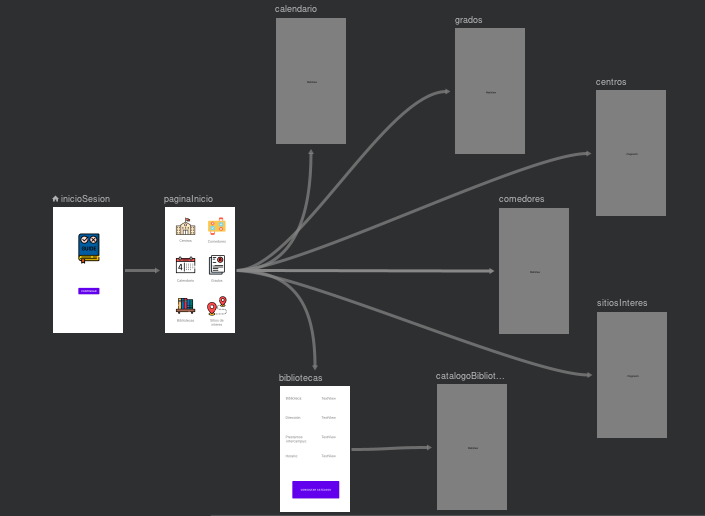
\includegraphics[width=\textwidth]{NavigationGraph.png}
	\caption{Grafo de navegación del proyecto}
\end{figure}


Como vemos, el proyecto comenzará en una pantalla de inicio en la que podremos seleccionar un centro, o decidir continuar sin seleccionar ninguno. Tras esto pasaremos a la pantalla principal, desde donde podremos pasar a las distintas secciones de la aplicación, que explicaremos en detalle en su respectiva sección.


